\documentclass[12pt]{article}

\usepackage[margin=1in]{geometry}
\usepackage{amsmath,amsthm,amssymb}
\usepackage{mathrsfs}
\usepackage{mathtools}
\usepackage{enumitem}
\usepackage{physics}
\usepackage{pdfpages}

\newcommand{\magsq}[1]{\big|#1\big|^2}
\newcommand{\avg}[1]{\left<#1\right>}

\begin{document}
	
\title{Homework 5}
\author{Sean Ericson \\ Phys 684}
\maketitle

\section*{Problem 1}
We start with the Maxwell wave equation
\[ \left(\vec{\nabla}^2-\frac{1}{c^2}\pdv[2]{t}\right)\vec{E}(\vec{r},t) = \mu_0\pdv[2]{t}\vec{P}(\vec{r}, t), \]
where
\[ \vec{E}(\vec{r},t) = \vec{E}_+(z,t) + \vec{E}_-(z,t); \quad \vec{E}_\pm(z,t) = \frac{1}{2}\hat{x}E_0(z,t)e^{\mp i\alpha(z,t)}, \]
\[ \vec{P}(\vec{r},t) = \vec{P}_+(z,t) + \vec{P}_-(z,t) = \frac{1}{2}\hat{x}\left(P_0(z,t)e^{-i\alpha(z,t)} + \text{c.c}\right), \]
\[ \alpha(z,t) = \omega t - kz - \phi(z,t), \]
and $E_0(z,t)\in\mathbb{R}$ while $P_0(z,t)\in\mathbb{C}$.
Noticing that
\begin{align*}
    2\pdv{z}\abs{E_\pm} &= \left(E_0' \mp iE_0\alpha'\right)e^{\mp i\alpha}, \\
    2\pdv{t}\abs{E_\pm} &= \left(\dot{E}_0 \mp iE_0\dot\alpha\right)e^{\mp i\alpha}, \\
    2\pdv{t}\abs{P_\pm} &= \left(\dot{P}_0 \mp P_0\dot\alpha\right)e^{\mp i\alpha} \\
    2\pdv[2]{t}\abs{P_\pm} &= \left(\ddot{P}_0 \mp \dot{P}_0\dot\alpha \mp P_0\ddot{\alpha} \mp i\dot{P}_0\dot\alpha + iP_0\dot\alpha^2\right)e^{\mp i\alpha} \\
    \alpha' &= -k - \phi' \\
    \dot\alpha &= \omega - \dot\phi,
\end{align*}
we factor the differential operator in the wave equation as 
\[ \partial_z^2 - \frac{1}{c^2}\partial_t^2 = \left(\partial_z + \frac{1}{c}\partial_t\right)\left(\partial_z - \frac{1}{c}\partial_t\right), \]
and begin applying it to the $\pm$ components of the fields:
\begin{align*}
    2\left(\partial_z - \frac{1}{c}\partial_t\right)\abs{E_\pm} &= \left[E_0' \mp iE_0\alpha' - \frac{1}{c}\left(\dot{E}_0 \mp iE_0\dot\alpha\right)\right]e^{\mp i\alpha} \\
    &= \left[\mp iE_0\left(\alpha' - \frac{1}{c}\dot\alpha\right) + E_0' - \frac{1}{c}\dot{E}_0\right]e^{\mp i\alpha} \\
    &= \left[\pm iE_0(2k + \phi' - \frac{1}{c}\dot\phi) + E_0' - \frac{1}{c}\dot{E}_0\right]e^{\mp i\alpha}.
\end{align*}
Now, in the slowly varying amplitude and phase approximation, we neglect terms proportional to $\ddot{E}_0$, $E_0''$, $\dot{P}_0$, and $\ddot{P}_0$.
So, as we apply the second half of the differential operator, let's drop the terms that will produce terms that we'll neglect anyway:
\begin{align*}
    2\left(\partial_z + \frac{1}{c}\partial_t\right)\left(\partial_z - \frac{1}{c}\partial_t\right)\abs{E_\pm} &\approx \pm2ik \left(\partial_z + \frac{1}{c}\partial_t\right)\left[E_0e^{\mp i\alpha}\right] \\
    &= \pm 2ik\left[E_0'  + \frac{1}{c}\dot{E}_0 \pm i\left(\phi' + \frac{1}{c}\dot\phi\right)\right]e^{\mp i\alpha}
\end{align*}
The other side of the wave equation is approximately
\[ \pdv[2]{t}P_0 \approx -\omega^2 P_0 \]
Equating the real and imaginary parts of each side of then gives the desired results.

\section*{Problem 2}
Starting with
\begin{align*}
    \dot{\tilde{\rho}}_{21} &= -(\gamma+i\delta) \tilde{\rho}_{21} + i \frac{\Omega_0}{2}\left(\rho_{22}-\rho_{11}\right) \\
    \dot{\rho}_{22} &= -\gamma_2\rho_{22} + \Re[i\Omega_0^*\tilde{\rho}_{21}],
\end{align*}
we first drop the tildes, then let $\rho_{21} = \frac{1}{2}(u - iv)$, and $\Omega_0 = \Omega_0' + i\Omega_0''$. Plugging these in, we get
\begin{alignat*}{3}
    &\quad & \frac{1}{2}(\dot{u} - i\dot{v}) &= -\frac{1}{2}(\gamma + i\delta)(u-iv) + \frac{i}{2}\left(\Omega_0' + i\Omega_0''\right)\left(2\rho_{22} - 1\right) \\
    &\quad & \dot{\rho}_{22} &= -\gamma_2\rho_{22} + \frac{1}{2}\left(\Omega_0'' u + \Omega_0' v\right) \\
    &\implies\quad & &  \\
    &\quad & \dot{u} &= -\gamma u - \delta v - 2\Omega_0''\rho_{22} + \Omega_0'' \\
    &\quad & \dot{v} &= -\delta u + \gamma v + 2\Omega_0' \rho_{22} - \Omega_0'  \\
    &\quad & \dot{\rho}_{22} &= \frac{\Omega_0''}{2} u + \frac{\Omega_0'}{2}v - \gamma_2\rho_{22}
\end{alignat*}
In the steady state, this is   
\[
\begin{rcases*}
    -\gamma u -\delta v - 2\Omega_0''\rho_{22} = -\Omega_0'' \\
    -\delta u + \gamma v + 2\Omega_0'\rho_{22} = \Omega_0' \\
    \frac{\Omega_0''}{2} u + \frac{\Omega_0'}{2} v - \gamma_2\rho_{22} = 0
\end{rcases*}
\implies
\mqty(-\gamma&-\delta&2\Omega_0''\\-\delta&+\gamma&2\Omega_0'\\\frac{\Omega_0''}{2}&\frac{\Omega_0'}{2}&-\gamma_2)\mqty(u\\v\\\rho_{22}) = \mqty(-\Omega_0''\\\Omega_0\\0)
\]
Inverting and solving, we find
\[ \mqty(u\\v\\\rho_{22}) = \frac{1}{\gamma^2 + \delta^2 + \frac{\gamma}{\gamma_2}\magsq{\Omega_0}}\mqty(\gamma\Omega_0'' - \delta\Omega_0' \\ \delta\Omega_0'' + \gamma\Omega_0' \\ \frac{\gamma\magsq{\Omega_0}}{2\gamma_2}). \]
Or, in terms of just density matrix components,
\begin{align*}
    \tilde{\rho}_{21} &= \frac{-\frac{1}{2}(\delta+i\gamma)\Omega_0}{\gamma^2 + \delta^2 + \frac{\gamma}{\gamma_2}\magsq{\Omega_0}} \\
    \rho_{22} &= \frac{\gamma\magsq{\Omega_0}}{2\gamma_2}\frac{1}{\gamma^2 + \delta^2 + \frac{\gamma}{\gamma_2}\magsq{\Omega_0}} \\
\end{align*}

\section*{Problem 3}
In lecture, we arrived at
\[ \chi(\omega) \approx \frac{N}{V}\frac{\mu^2}{\epsilon_0\hbar}\frac{\rho_{22}^{(0)} - \rho_{11}^{(0)}}{\delta - i \gamma}, \]
where we used the first order approximation 
\[ \rho_{21}^{(1)} \approx \frac{\Omega_0}{2}\frac{\rho_{22}^{(0)}-\rho_{11}^{(0)}}{\delta - i\gamma}. \]
If I use the full solution that I got in the previous problem, however, I get an imaginary component of $\chi$ that is
\[ \chi'' = \frac{N}{V}\frac{\mu^2}{\epsilon_0\hbar}\frac{\gamma}{\gamma^2 + \delta^2 + \frac{\gamma}{\gamma_2}\magsq{\Omega_0}}, \]
which is the same up to that extra term in the denominator. That extra term seems to mess up the simplification when we set $\delta =0\;(\implies \omega = \omega_0)$, $\gamma = \gamma_2/2$, and
\[ \gamma_2 = \frac{\mu^2\omega_0^3}{3\pi \epsilon_0\hbar c^3}. \]
If we ignore it, then everything goes through exactly as it did in lecture. When we compare 
\[ \alpha = \frac{\omega}{c}\chi'' = \frac{N}{V}\sigma, \]
we get
\[ \sigma = \frac{c^2}{\omega_0^2}6\pi = \frac{3}{2\pi}\lambda_0^2 \]
Given
\begin{align*}
    \frac{N}{V} = 3\times10^9\;\frac{\text{atoms}}{\text{cm}^3} \\
    \gamma_2 = 2\pi\times10\;\text{MHz} \\
    \lambda_0 = 600\;\text{nm}
\end{align*}
we have that 
\[ \alpha = \frac{N}{V}\frac{3}{2\pi}\lambda_0^2 \]
\begin{enumerate}[label=(\alph*)]
    \item \[ n + 1 + \frac{1}{2}\chi' \]
\end{enumerate}

\section*{Problem 4}
\begin{enumerate}[label=(\alph*)]
    \item The rate equation approximation seems to be valid in the first and third cases.
    It's clearly not valid in the second case, as the coherence is almost exactly $90^\circ$ out of phase with the population
\end{enumerate}

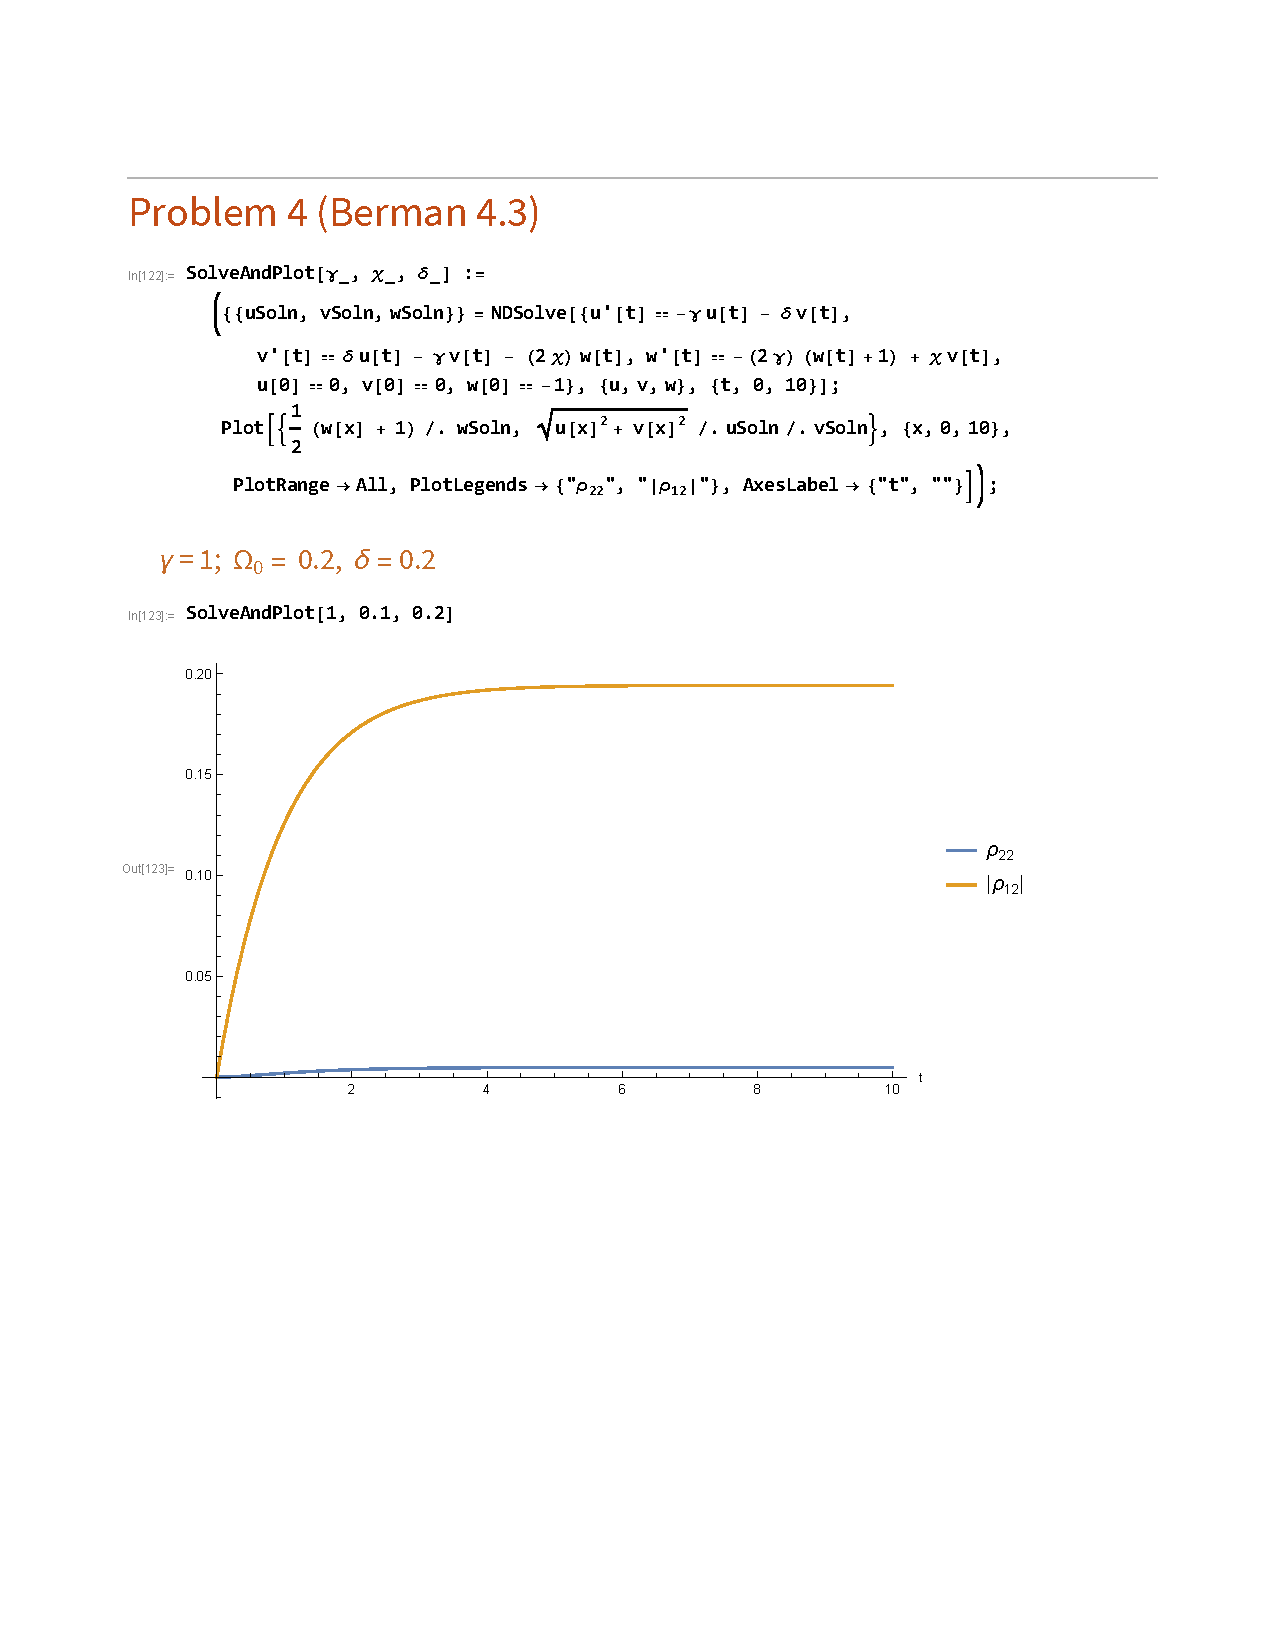
\includepdf[pages=-]{calcs/HW5_mathematica.pdf}
\end{document}